\documentclass[journal=jacsat,manuscript=article]{achemso}
\usepackage[version=3]{mhchem}
\usepackage{amsmath}
\newcommand*\mycommand[1]{\texttt{\emph{#1}}}
\author{Rahmi Chowdhury}
\affiliation{Department of Chemistry and Biology, Toronto Metropolitan
University,}
\email{rchowdhury@ryerson.ca}

\abbreviations{IR,NMR,UV}

\keywords{American Chemical Society, \LaTeX}

\title[An \textsf{achemso} demo]{Analytical Insights into Thirteen OPE
Variables}
\makeatletter
\ifxetex
  \usepackage[setpagesize=false, % page size defined by xetex
              unicode=false, % unicode breaks when used with xetex
              xetex]{hyperref}
\else
  \usepackage[unicode=true]{hyperref}
\fi
\hypersetup{breaklinks=true,
            bookmarks=true,
            pdfauthor={},
            pdftitle={},
            colorlinks=true,
            urlcolor=blue,
            linkcolor=magenta,
            pdfborder={0 0 0}}
\urlstyle{same}  % don't use monospace font for urls


% tightlist command for lists without linebreak
\providecommand{\tightlist}{%
  \setlength{\itemsep}{0pt}\setlength{\parskip}{0pt}}

% From pandoc table feature
\usepackage{longtable,booktabs,array}
\usepackage{calc} % for calculating minipage widths
% Correct order of tables after \paragraph or \subparagraph
\usepackage{etoolbox}
\makeatletter
\patchcmd\longtable{\par}{\if@noskipsec\mbox{}\fi\par}{}{}
\makeatother
% Allow footnotes in longtable head/foot
\IfFileExists{footnotehyper.sty}{\usepackage{footnotehyper}}{\usepackage{footnote}}
\makesavenoteenv{longtable}



\begin{document}
\begin{abstract}
There are many different parameters that play an integral roll in
predictive Organophosphate Esters (OPEs) modelling. Much of this
research has revolved around using various physical and chemical
properties to determine the Overall Persistance(POV) and Long-Range
Transport Potential (LRTP) of these organic chemicals at a screening.
While these models have been incredibly beneficial, I wanted to look for
ways to better help the predictive patterning of OPEs.To do this, some
questions this paper looked to answer was 1) is there a correlation
between any of the variables present? 2) How can these relationships (if
any) help to improve predictability of OPEs. With that being said, this
paper looked to create a basis point for these predictive tools to
better understand the relationships between all these parameters. This
paper analyzed all the current known available data about each of these
parameters for 10 known native OPEs
(TPP,TMTP,TPTP,TEP,TPrP,TBP,TBEP,EHDP,TCEP,TCPP) and compared them to
one another to see if any sort of relationship can be found. The 14
parameters looked at include: mass, Characteristic Travel Distance in
air (CTD\_a), Characteristic Travel Distance in water (CTD\_w),
POV\_air, POV\_water, Number of Carbon units (C), Number of Hydrogen
units(H), Number of Chlorine units(Cl), Number of Oxygen units(O),
number of Phosphorus(Ph), air-water coefficient from the
literature(KAW), octanol-water coefficient from the literature(KOW), and
octanol-air coefficient from the literature(KOA), Retention Time (RT).
Using the pearson test, the most statistically signiifcant results
include the: POV\_w-CTD\_w pair,CTD\_a-KOA,H-KOA , KAW-POV\_a at higher
masses, KOW-RT at lower masses,and KOA-mass, they each had values of
0.999,-0.944,0.952,-0.997,0.952, and 0.910 respectively. These
relationships are incredibly important because it aids in giving
valuable inisght when it comes to predicting the behavior of similar
OPEs. Some noteworthy relationships that may come in aid is the strong
correlation between KOA values of OPEs and their respective masses. This
relationship can help help predict the extent of the LRTP of OPEs.
\end{abstract}
\begin{tocentry}
Some journals require a graphical entry for the Table of Contents.
This should be laid out ``print ready'' so that the sizing of the
text is correct.

Inside the \texttt{tocentry} environment, the font used is Helvetica
8\,pt, as required by \emph{Journal of the American Chemical
Society}.

The surrounding frame is 12\,cm by 5\,cm, which is the maximum
permitted for  \emph{Journal of the American Chemical Society}
graphical table of content entries. The box will not resize if the
content is too big: instead it will overflow the edge of the box.

This box and the associated title will always be printed on a
separate page at the end of the document.
\end{tocentry}

\hypertarget{chapter-1-introduction-the-history-of-opes}{%
\section{Chapter 1: Introduction The History of
OPEs}\label{chapter-1-introduction-the-history-of-opes}}

Organophosphate Esters (OPEs) have been found all across the world. In
food webs through bioaccumulation(Du et al., 2019), in sediments(Chokwe
et al., 2020), in people via absorption, in the air and in the waters up
north in the Arctic through various modes of transport (Castro-Jiménez
et al., 2014) (Möller et al., 2011) (Sühring et al., 2016)(Salamova et
al., 2013) (Salamova et al., 2013) (Luo et al., 2016) (Lai et al.,
2015). Recent research suggests these OPEs have persistent organic
pollutant (POPs)-like characteristics (Guigueno \& Fernie, 2017). While
on the human side, studies have shown that some OPEs can potentially be:
mutagenic, carcinogenic, genotoxic and neurotoxic (Zhao et al., 2020).
OPEs have the potential to be harmful, also ever since PBDEs were
banned, the consumption of these dangerous chemicals has greatly
increased (Chupeau et al., 2020). Originally, due to a combination of
physio-chemical property assessments and a lack of observational data,
OPEs were thought to have been a safe substitute. According to the
Danish EPA in the EU Risk Assessment they found that TPP (an OPE) didn't
appear to have a greater negative impact than the other flame retardants
(FRs) they were using at the time (Pakalin et al., 2007). Other research
has also used this same argument, citing that OPEs do not meet the
criteria listed out by the Stockholm Convention to be as harmful as the
now restricted/banned polybrominated diphenyl ethers (PBDEs) that they
are replacing(Fiedler et al., 2019). Under the Stockholm convention
there are 4 key criteria listed to be qualified as persistent organic
pollutants (POPs) they are: 1) persistence potential i.e persists in the
environment and is resistant to degradation, 2) bioaccumulation
potential i.e each chemical's potential to accumulate within various
organisms, 3) their long-range transport potential (LRTP) i.e the
chemical's ability to propagate itself beyond local release locations
and 4) Toxicity (Fiedler et al., 2019). The criterion is determined by
both observational data and modelling tools. At the time of writing
there are modelling tools that underestimate the POP like capabilities
of OPEs (Sühring et al., 2020). While on the observational side, it is
becoming apparent that OPEs share POP-like characteristics; for example
one study found that OPEs persist in indoor dust and bioaccumulate
within humans (Y. Wang et al., 2021). Part of these issues in properly
predicting POP like properties of OPEs may be attributed to the
modelling tools used to assess OPEs. Default parameters of tools such as
the Organization of Economic Co-operation and Development (OECD)
Persistance (POV) and LRTP Screening Tool (``The Tool'') underestimated
both the POV and LRTP values for OPEs(Sühring et al., 2020). This is
incredibly alarming as predictive modelling tools such as the OECD and
POV Screening tool uses data such as OPEs having have half-lives of less
than 2 days in air to predict LRTP. Simply based on the knowledge of OPE
half-lives being less than 2 days in air, the sheer notion that these
OPEs could be found in remote places such as the Arctic would be absurd;
and yet emerging data clearly attests to this (Sühring et al,
2021)(Sühring et al., 2016). One way this disparity can be sufficiently
explained then is through aerosol absorption. By absorbing into aerosols
those same OPEs now had a mode of transport over long ranges (Möller et
al., 2012). As noted by Möller et al the half lives presented is only
within the gaseous state, this is a factor that must be analyzed more
thoroughly to better understand the half-lives of OPEs not just in the
gaseous state, but when adsorbed to other aerosols.

\hypertarget{chapter-2-oecd-and-pov-screening-tool}{%
\section{Chapter 2: OECD and POV Screening
TOol}\label{chapter-2-oecd-and-pov-screening-tool}}

One commonly used assessment tool for LRTP and toxicity is the OECD POV
and LRTP Screening Tool (The Tool). Designed with extensive research of
PBDEs and other POPs in mind the Tool was parameterized to estimate the
persistence and LRTP of POPs but would come short in adequately
quantifying the persistence and LRTP of many more hydrophilic OPFRs
(Zhang and Sühring et al., 2016). Multiple comparative models between
The Tool and other models have begun to show the limitations of said
parameters. One study found that the poly parameter linear free energy
relationships (ppLFERs) tool had the ability to improve the current
gas-particle partitioning description for polar chemicals(CW et al.,
2008). Another study found that by including other environmental
parameters such as wind speed had a significant effect on LRTP(Zhu et
al., 2014). Clearly from this it can be seen that the tool must be
updated, its ability to predict the fate of OPEs must be broadened as
all parameters must be reassessed. This is the goal that this paper
sought out attempted to solve as it can be seen throughout the rest of
this paper.

\hypertarget{chapter-3-figures-and-results}{%
\section{Chapter 3 Figures and
Results}\label{chapter-3-figures-and-results}}

\begin{longtable}[]{@{}
  >{\raggedright\arraybackslash}p{(\columnwidth - 28\tabcolsep) * \real{0.0556}}
  >{\centering\arraybackslash}p{(\columnwidth - 28\tabcolsep) * \real{0.1111}}
  >{\centering\arraybackslash}p{(\columnwidth - 28\tabcolsep) * \real{0.0889}}
  >{\centering\arraybackslash}p{(\columnwidth - 28\tabcolsep) * \real{0.0778}}
  >{\centering\arraybackslash}p{(\columnwidth - 28\tabcolsep) * \real{0.0778}}
  >{\centering\arraybackslash}p{(\columnwidth - 28\tabcolsep) * \real{0.0778}}
  >{\centering\arraybackslash}p{(\columnwidth - 28\tabcolsep) * \real{0.0444}}
  >{\centering\arraybackslash}p{(\columnwidth - 28\tabcolsep) * \real{0.0444}}
  >{\centering\arraybackslash}p{(\columnwidth - 28\tabcolsep) * \real{0.0444}}
  >{\centering\arraybackslash}p{(\columnwidth - 28\tabcolsep) * \real{0.0333}}
  >{\centering\arraybackslash}p{(\columnwidth - 28\tabcolsep) * \real{0.0444}}
  >{\centering\arraybackslash}p{(\columnwidth - 28\tabcolsep) * \real{0.0778}}
  >{\centering\arraybackslash}p{(\columnwidth - 28\tabcolsep) * \real{0.0667}}
  >{\centering\arraybackslash}p{(\columnwidth - 28\tabcolsep) * \real{0.0667}}
  >{\centering\arraybackslash}p{(\columnwidth - 28\tabcolsep) * \real{0.0889}}@{}}
\caption{Summary of OPE Data}\tabularnewline
\toprule()
\begin{minipage}[b]{\linewidth}\raggedright
OPEs
\end{minipage} & \begin{minipage}[b]{\linewidth}\centering
mass
\end{minipage} & \begin{minipage}[b]{\linewidth}\centering
CTD\_a
\end{minipage} & \begin{minipage}[b]{\linewidth}\centering
CTD\_w
\end{minipage} & \begin{minipage}[b]{\linewidth}\centering
POV\_a
\end{minipage} & \begin{minipage}[b]{\linewidth}\centering
POV\_w
\end{minipage} & \begin{minipage}[b]{\linewidth}\centering
H
\end{minipage} & \begin{minipage}[b]{\linewidth}\centering
C
\end{minipage} & \begin{minipage}[b]{\linewidth}\centering
Cl
\end{minipage} & \begin{minipage}[b]{\linewidth}\centering
O
\end{minipage} & \begin{minipage}[b]{\linewidth}\centering
Ph
\end{minipage} & \begin{minipage}[b]{\linewidth}\centering
KAW
\end{minipage} & \begin{minipage}[b]{\linewidth}\centering
KOW
\end{minipage} & \begin{minipage}[b]{\linewidth}\centering
KOA
\end{minipage} & \begin{minipage}[b]{\linewidth}\centering
RT
\end{minipage} \\
\midrule()
\endfirsthead
\toprule()
\begin{minipage}[b]{\linewidth}\raggedright
OPEs
\end{minipage} & \begin{minipage}[b]{\linewidth}\centering
mass
\end{minipage} & \begin{minipage}[b]{\linewidth}\centering
CTD\_a
\end{minipage} & \begin{minipage}[b]{\linewidth}\centering
CTD\_w
\end{minipage} & \begin{minipage}[b]{\linewidth}\centering
POV\_a
\end{minipage} & \begin{minipage}[b]{\linewidth}\centering
POV\_w
\end{minipage} & \begin{minipage}[b]{\linewidth}\centering
H
\end{minipage} & \begin{minipage}[b]{\linewidth}\centering
C
\end{minipage} & \begin{minipage}[b]{\linewidth}\centering
Cl
\end{minipage} & \begin{minipage}[b]{\linewidth}\centering
O
\end{minipage} & \begin{minipage}[b]{\linewidth}\centering
Ph
\end{minipage} & \begin{minipage}[b]{\linewidth}\centering
KAW
\end{minipage} & \begin{minipage}[b]{\linewidth}\centering
KOW
\end{minipage} & \begin{minipage}[b]{\linewidth}\centering
KOA
\end{minipage} & \begin{minipage}[b]{\linewidth}\centering
RT
\end{minipage} \\
\midrule()
\endhead
TPP & 327.0781 & 584.00 & 65 & 2 & 39 & 18 & 15 & 0 & 4 & 1 & 0.53 &
6.34 & NA & 14.554 \\
TMTP & 369.1250 & 278.52 & 64 & 1 & 39 & 21 & 21 & 0 & 4 & 1 & 0.53 &
6.34 & NA & 17.902 \\
TPTP & 369.1250 & 584.00 & 65 & 2 & 39 & 21 & 21 & 0 & 4 & 1 & 0.53 &
6.34 & NA & 18.091 \\
TEP & 183.0781 & 155.00 & 24 & 0 & 14 & 6 & 15 & 0 & 4 & 1 & -4.60 &
0.90 & 5.5 & 10.848 \\
TPrP & 225.1250 & 107.00 & 26 & 0 & 15 & 9 & 21 & 0 & 4 & 1 & 0.29 &
1.87 & NA & 14.074 \\
TBP & 267.1720 & 101.00 & 7 & 0 & 4 & 12 & 27 & 0 & 4 & 1 & -5.80 & 4.20
& 10.0 & 16.540 \\
TBEP & 399.2506 & 8.00 & 28 & 21 & 16 & 18 & 39 & 0 & 7 & 1 & -9.30 &
3.00 & 12.3 & 17.076 \\
EHDP & 363.1720 & 201.00 & 28 & 1 & 16 & 20 & 27 & 0 & 4 & 1 & 0.58 &
6.30 & NA & 18.616 \\
TCEP & 284.9612 & NA & NA & NA & NA & 6 & 12 & 3 & 4 & 1 & -6.00 & 1.60
& 7.6 & 12.969 \\
TCPP & 327.0081 & 179.00 & 88 & 1 & 51 & 9 & 11 & 4 & 4 & 1 & 0.27 &
2.59 & NA & 14.565 \\
\bottomrule()
\end{longtable}

\hypertarget{table-results}{%
\section{3.1 Table Results}\label{table-results}}

As it can be seen from the table, there are a total of 14 variables
being compared to here for the given 10 OPEs. Not all data was present
for each OPE so some appear blank.

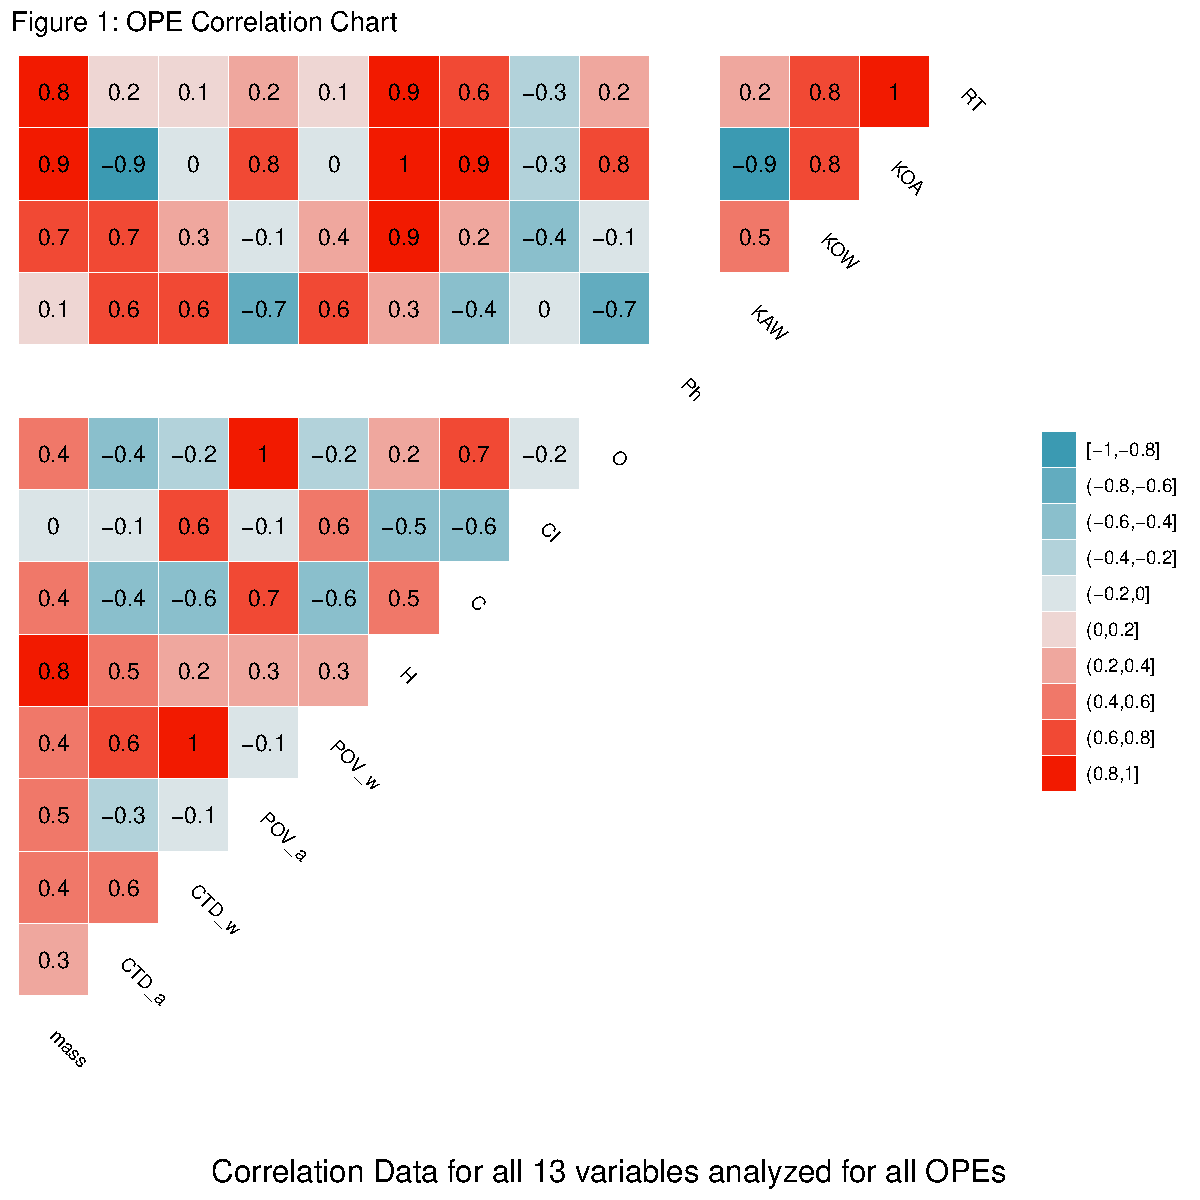
\includegraphics{Rahmi_Chowdhury_500621744_Final_project_files/figure-latex/unnamed-chunk-3-1.pdf}

\hypertarget{chart-results}{%
\section{3.2 Chart Results}\label{chart-results}}

An easy to read summary data chart of the correlation potential between
the OPE variables. The chart starts with mass on the left, all the way
down to RT on the right. The chart was broken down into 10 categories of
correlation values, with +/-(0.8,1) having the highest degree of
absolute coefficients. Due to rounding to 1 significant digit some
values have a complete correlation.

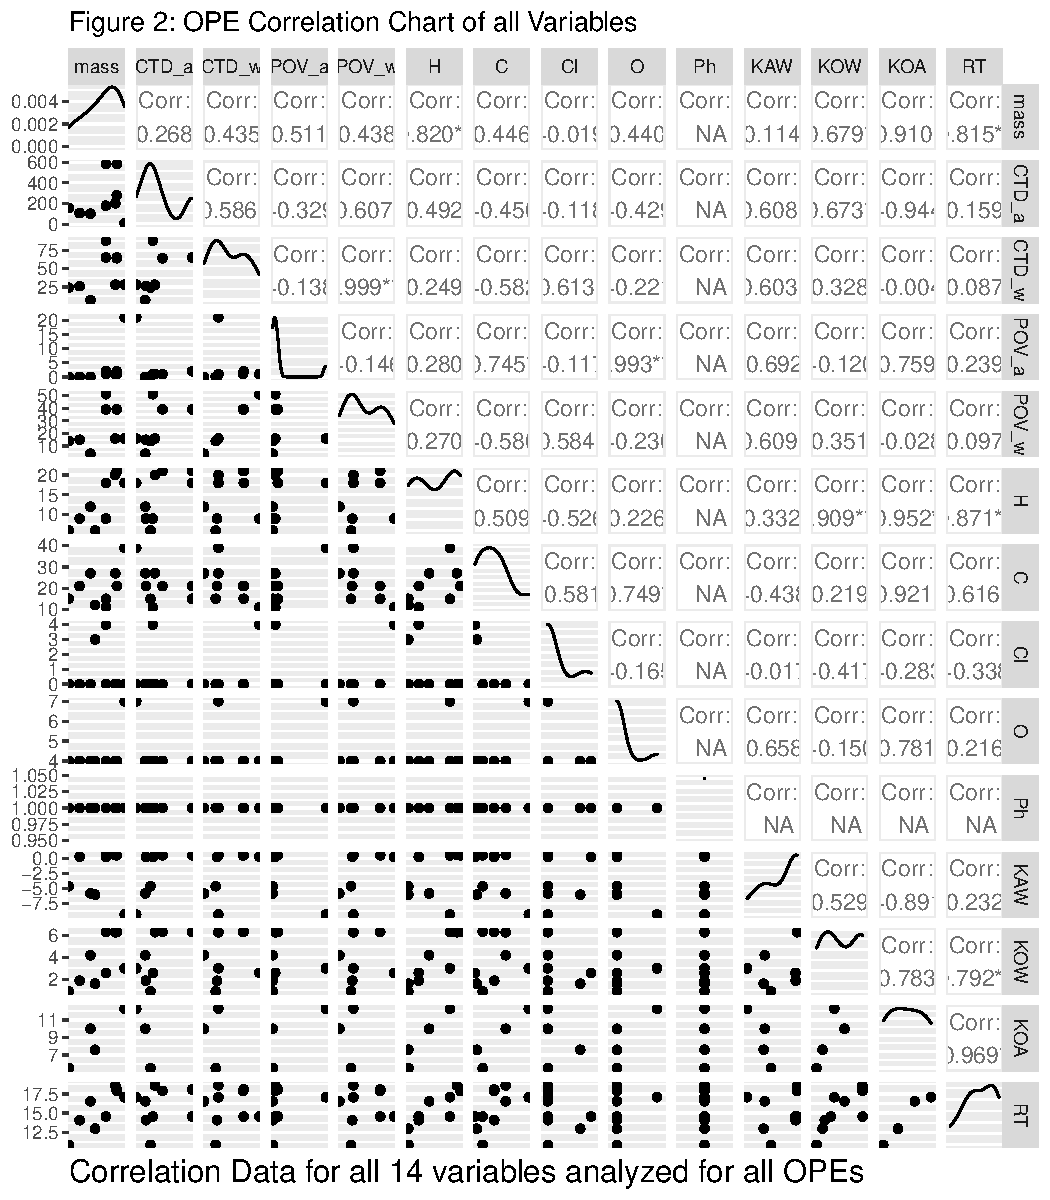
\includegraphics{Rahmi_Chowdhury_500621744_Final_project_files/figure-latex/unnamed-chunk-4-1.pdf}

\hypertarget{ggpairs-ope-correlation-data.}{%
\section{3.3 GGPairs OPE Correlation
Data.}\label{ggpairs-ope-correlation-data.}}

Here we can see the total analysis of all the OPEs pitted against each
other. Due to the sheer number of variables it becomes difficult to read
so this chart is simply used as a demonstration. More comprehensive
graphs are designed below breaking down the variables within smaller
categories

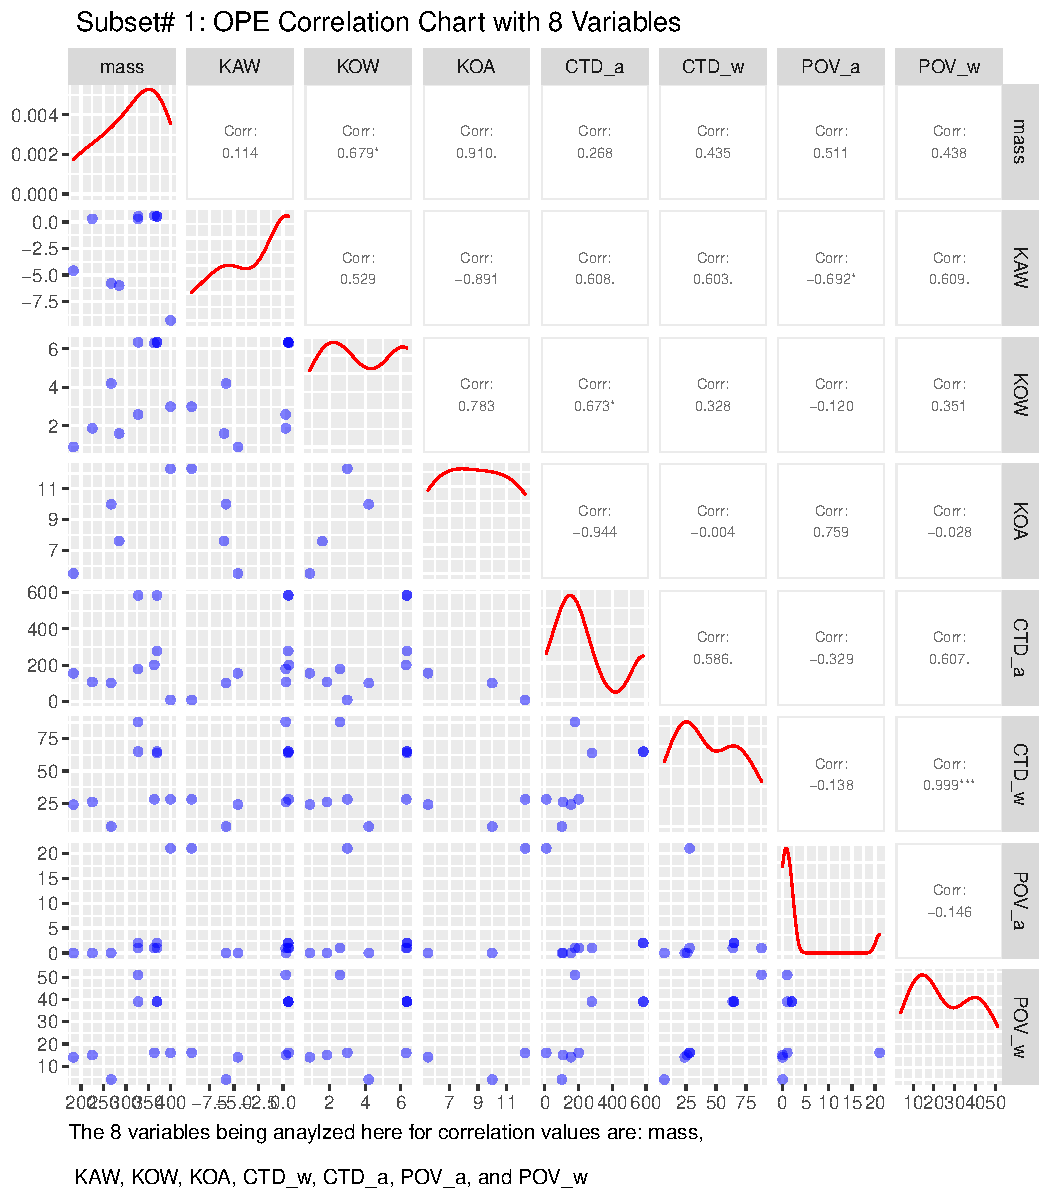
\includegraphics{Rahmi_Chowdhury_500621744_Final_project_files/figure-latex/unnamed-chunk-5-1.pdf}
\# 3.4 GGPlots Subset Chart 1. This subset compares KAW, KOW, KOA,
CTD\_w, CTD\_a, POV\_a,POV\_w, and mass. Some notable values here are
between the pairs: CTD\_w-POV\_w, KOA-mass,KOA-KAW, and CTD\_a-KOA with
values: 0.999,0.910,-0.891 and -0.944 respectively.

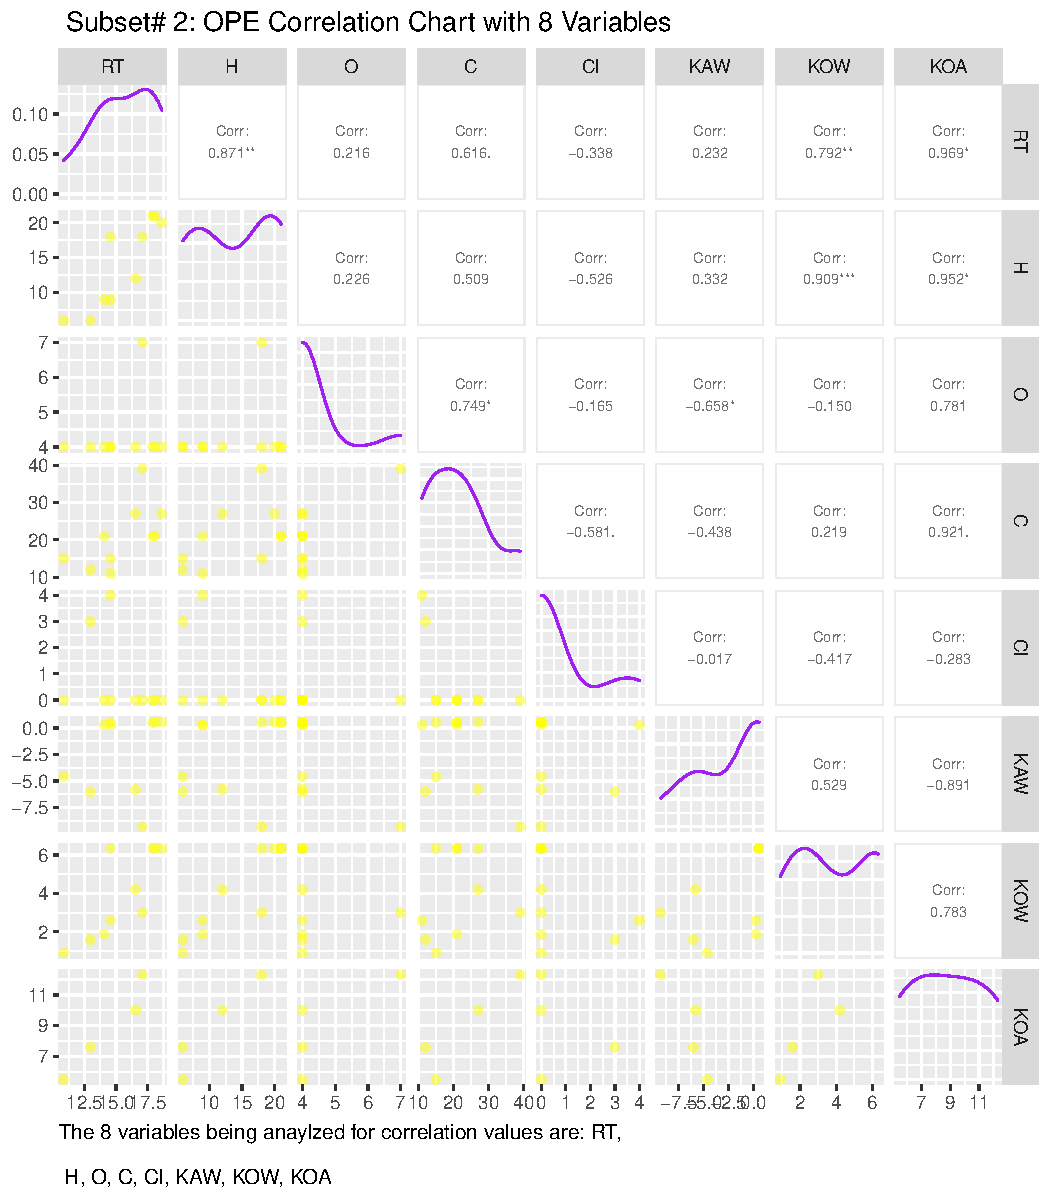
\includegraphics{Rahmi_Chowdhury_500621744_Final_project_files/figure-latex/unnamed-chunk-6-1.pdf}
\# 3.5 GGPlots Subset Chart 2. This subset compares
``RT'',``H'',``O'',``C'',``Cl'', ``KAW'', ``KOW'', and ``KOA''. Some
notable pairs here not already previously mentioned are:
KOA-RT,KOA-H,KOA-C, and KOW-H, with values: 0.969,0.952,0.921, and 0.909
respectively. \#note how significant this is because the pairs KOA-H and
KOA-C may be a good predictive factor for what mode of transport other
similar OPEs may use. With OPEs high in Carbon, oxygen and hydrogen
likely to be in air while not so much in water. While OPEs with Cl have
a higher likely hood of using water as their mode of transport

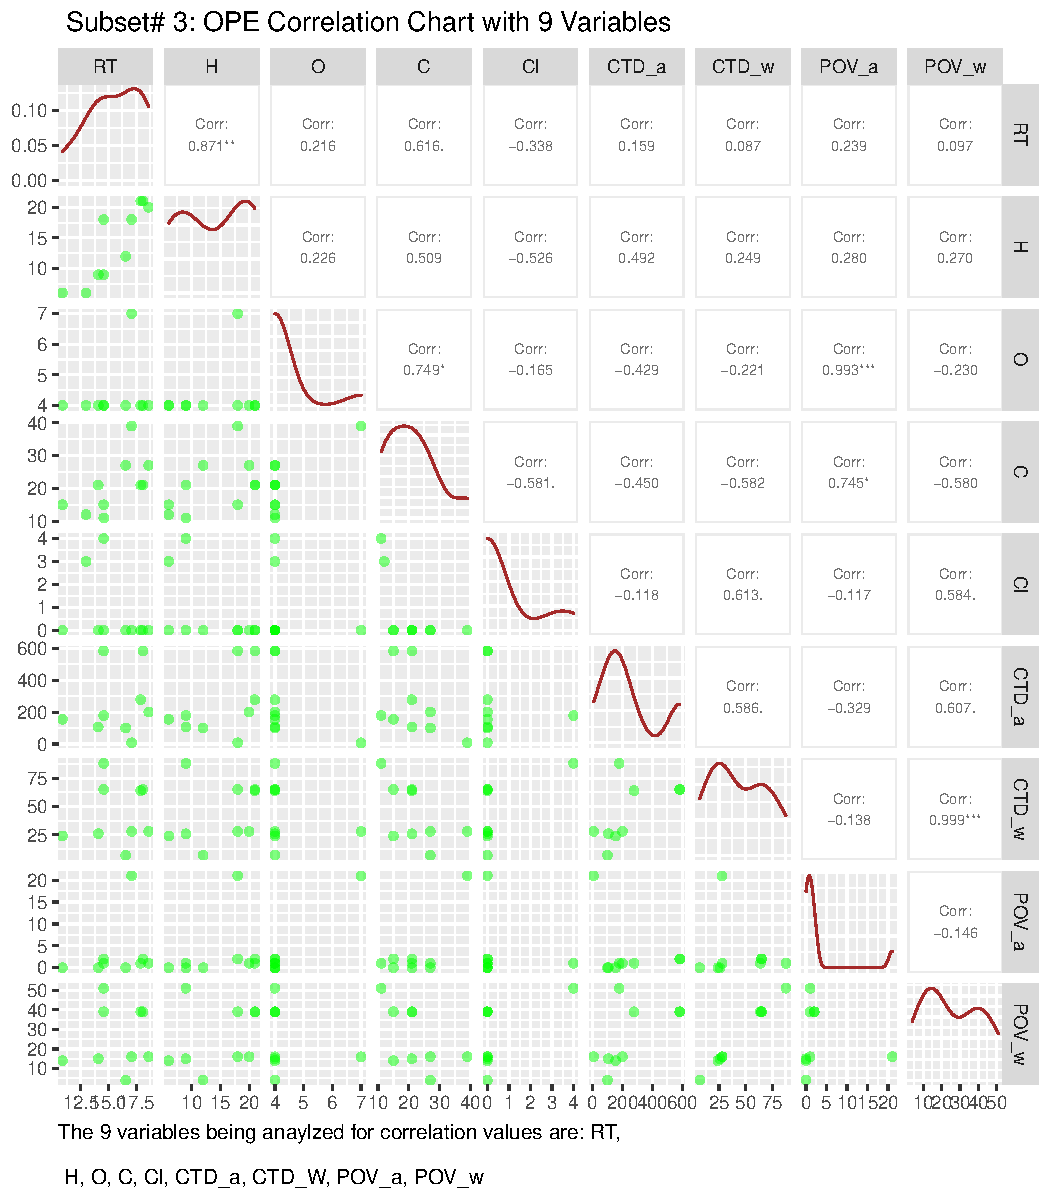
\includegraphics{Rahmi_Chowdhury_500621744_Final_project_files/figure-latex/unnamed-chunk-7-1.pdf}
\# 3.6 GGPlots Subset Chart 3. This subset compares
RT'',``H'',``O'',``C'',``Cl'', ``CTD\_a'', ``CTD\_w'',
``POV\_a'',``POV\_w''. The main point of this subset is to compare the
chemical compositions with the POV. Some notable pairs here not already
previously mentioned are: POV\_a-POV\_w, and POV\_a-O, with values:
0.999, 0.993 respectively. \#note how significant this is, the POV\_a
match up with O at such a high value matches up with its CTD\_a-O as
well. Showing that O is an indicator of both and likely needed for
atmospheric transport

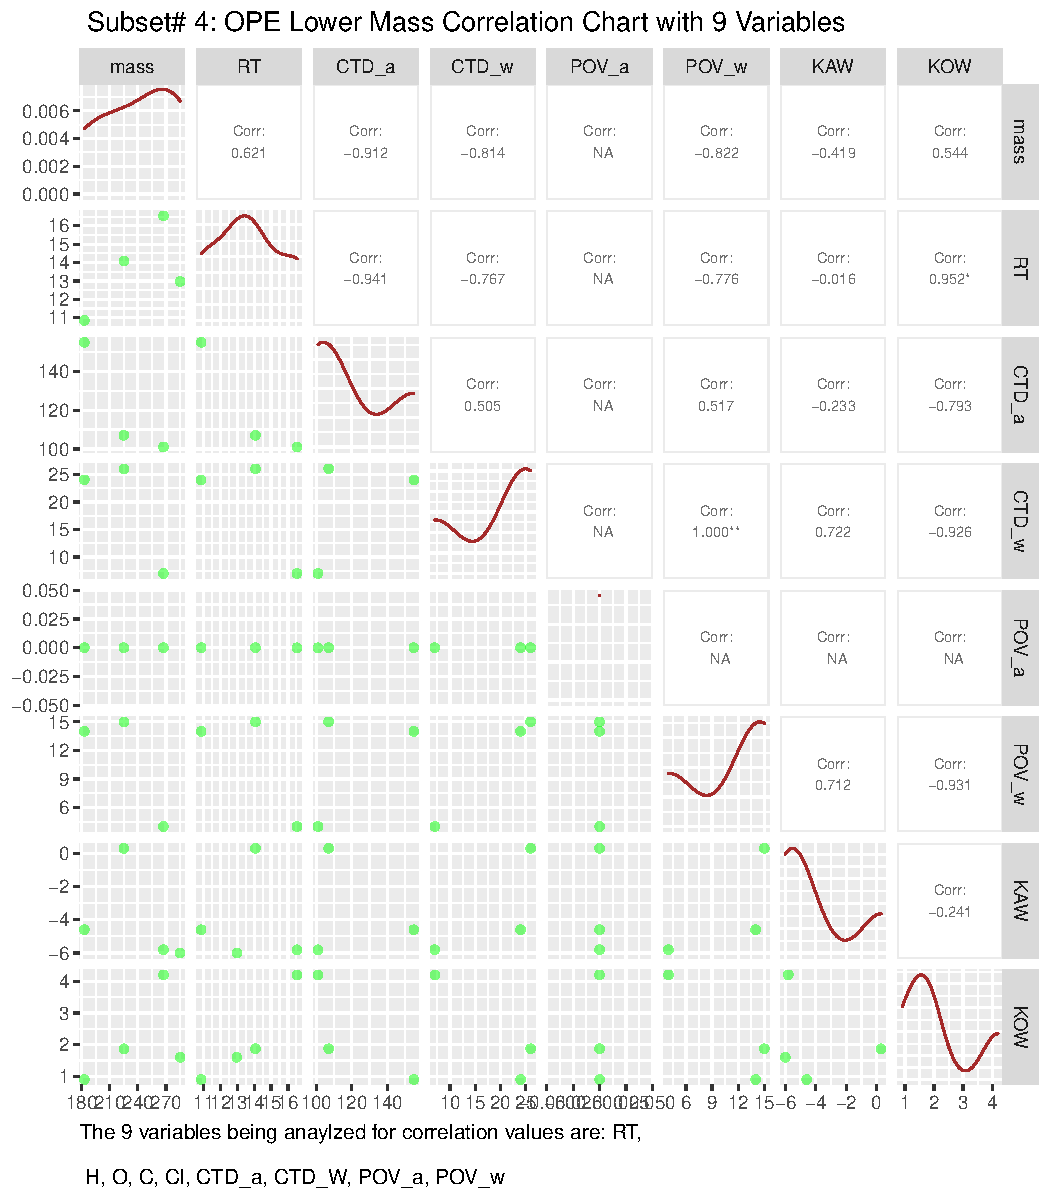
\includegraphics{Rahmi_Chowdhury_500621744_Final_project_files/figure-latex/unnamed-chunk-8-1.pdf}
\# 3.7 GGPlots Subset Chart 4. This subset compares ``mass'',``RT'',
``CTD\_a'', ``CTD\_w'', ``POV\_a'',``POV\_w'',``KAW'',``KOW''. Due to
the absence in all data for each OPE, this data is less accurate for the
representation of OPEs with a mass less than 300. Despite this,some
notable pairs here are: KOW-RT(0.952),KOW-CTD\_w (-0.926),
KOW-POV\_w(-0.931), CTD\_a-mass(-0.912),and CTD\_a-RT(-0.941) with
values: 0.952, -0.926,-0.931,-0.912,-0.941 respectively.

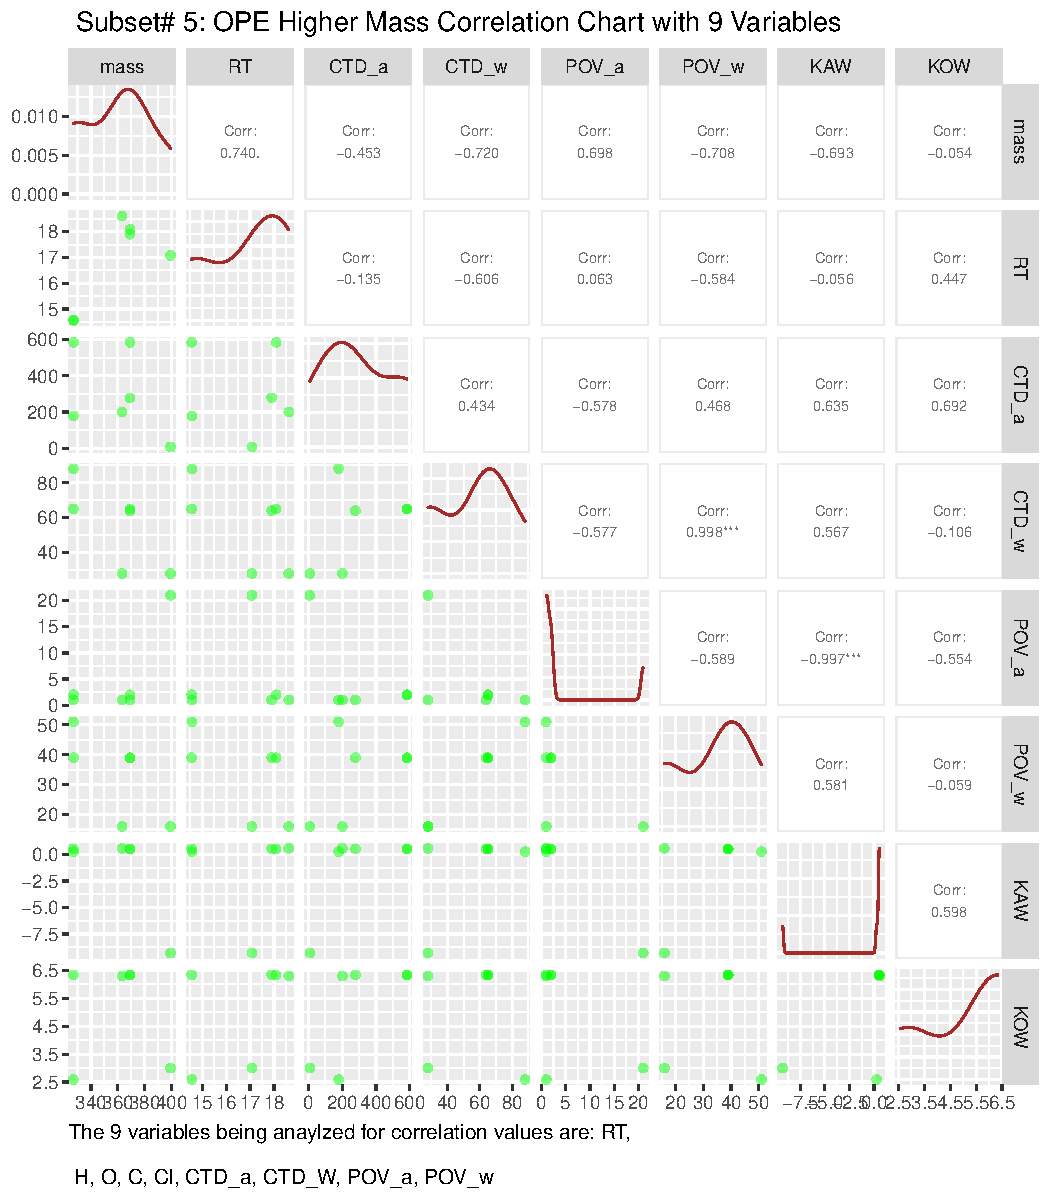
\includegraphics{Rahmi_Chowdhury_500621744_Final_project_files/figure-latex/unnamed-chunk-9-1.pdf}
\# 3.8 GGPlots Subset Chart 5. This subset compares ``mass'',``RT'',
``CTD\_a'', ``CTD\_w'', ``POV\_a'',``POV\_w'',``KAW'',``KOW''. Due to
the absence in all data for each OPE, this data is less accurate for the
representation of OPEs with a mass over 300. Despite this,some notable
pairs here are: POV\_a-KAW, and POV\_w-CTD\_w with values: -0.997 and
0.998 respectively.

\hypertarget{conclusion-and-discussion}{%
\section{Conclusion and Discussion}\label{conclusion-and-discussion}}

As noted throughout the entirety of the results, many of the variables
within the OPE parameters have some sort of relationship with each
other, whether that be positive or negative. Looking deeper into these
results in section 3.5 note how significant the statistical relationship
is between the pairs KOA-H and KOA-C. This is important because it may
be a good predictive factor for what mode of transport other similar
OPEs with high units of hydrogen and carbon atoms may use. Implying that
OPEs high in Carbon, oxygen and hydrogen likely to be in air while not
so much in water. Section 3.5 also highlights to a lesser degree that
OPEs with Cl have a higher likely hood of using water as their mode of
transport.In section 3.6 there was also another pair with statistical
significance: POV\_a-O. This is because it supports the previous
findings of 3.5, higher concentrations of oxygen have a strong positive
coefficient value with the overall persistence of the OPE in air.
Implying once more that this type of OPE is more likely to use an
atmospheric mode of transport. This adds evidence to the fact that
specific compounds may be indicators for certain modes of
transports.These results are profound in that sense that when isolated
for each significant relationship a crude model can be made to predict
future OPEs. Future work I would love to do is to attempt these concepts
on other OPEs to see how well it stands up, as well as expand the
database to get more accurate results.

\hypertarget{references}{%
\subsection{References}\label{references}}

Castro-Jiménez, J., Berrojalbiz, N., Pizarro, M., \& Dachs, J. (2014).
Organophosphate ester (OPE) flame retardants and plasticizers in the
open Mediterranean and Black Seas atmosphere. Environmental Science \&
Technology, 48(6), 3203--3209. https://doi.org/10.1021/ES405337G

Chokwe, T. B., Abafe, O. A., Mbelu, S. P., Okonkwo, J. O., \& Sibali, L.
L. (2020). A review of sources, fate, levels, toxicity, exposure and
transformations of organophosphorus flame-retardants and plasticizers in
the environment. Emerging Contaminants, 6, 345--366.
https://doi.org/10.1016/J.EMCON.2020.08.004

Chupeau, Z., Bonvallot, N., Mercier, F., Bot, B. Le, Chevrier, C., \&
Glorennec, P. (2020). Organophosphorus Flame Retardants: A Global Review
of Indoor Contamination and Human Exposure in Europe and Epidemiological
Evidence. International Journal of Environmental Research and Public
Health, 17(18), 1--24. https://doi.org/10.3390/IJERPH17186713

CW, G., M, S., M, M., F, W., U, S., \& K, H. (2008). Dependence of
persistence and long-range transport potential on gas-particle
partitioning in multimedia models. Environmental Science \& Technology,
42(10), 3690--3696. https://doi.org/10.1021/ES702619P

Du, J., Li, H., Xu, S., Zhou, Q., Jin, M., \& Tang, J. (2019). A review
of organophosphorus flame retardants (OPFRs): occurrence,
bioaccumulation, toxicity, and organism exposure. Environmental Science
and Pollution Research, 26(22), 22126--22136.
https://doi.org/10.1007/S11356-019-05669-Y/FIGURES/2

Fiedler, H., Kallenborn, R., Boer, J. de, \& Sydnes, L. K. (2019). The
Stockholm Convention: A Tool for the Global Regulation of Persistent
Organic Pollutants. Chemistry International, 41(2), 4--11.
https://doi.org/10.1515/CI-2019-0202

Guigueno, M. F., \& Fernie, K. J. (2017). Birds and flame retardants: A
review of the toxic effects on birds of historical and novel flame
retardants. Environmental Research, 154, 398--424.
https://doi.org/10.1016/J.ENVRES.2016.12.033

Lai, S., Xie, Z., Song, T., Tang, J., Zhang, Y., Mi, W., Peng, J., Zhao,
Y., Zou, S., \& Ebinghaus, R. (2015). Occurrence and dry deposition of
organophosphate esters in atmospheric particles over the northern South
China Sea. Chemosphere, 127, 195--200.
https://doi.org/10.1016/J.CHEMOSPHERE.2015.02.015

Luo, P., Bao, L. J., Guo, Y., Li, S. M., \& Zeng, E. Y. (2016).
Size-dependent atmospheric deposition and inhalation exposure of
particle-bound organophosphate flame retardants. Journal of Hazardous
Materials, 301, 504--511. https://doi.org/10.1016/J.JHAZMAT.2015.09.014

Möller, A., Xie, Z., Caba, A., Sturm, R., \& Ebinghaus, R. (2011).
Organophosphorus flame retardants and plasticizers in the atmosphere of
the North Sea. Environmental Pollution, 159(12), 3660--3665.
https://doi.org/10.1016/J.ENVPOL.2011.07.022

Möller, A., Sturm, R., Xie, Z., Cai, M., He, J., \& Ebinghaus, R.
(2012). Organophosphorus Flame Retardants and Plasticizers in Airborne
Particles over the Northern Pacific and Indian Ocean toward the Polar
Regions: Evidence for Global Occurrence. Environmental Science and
Technology, 46(6), 3127--3134. https://doi.org/10.1021/ES204272V

Pakalin, S., Cole, T., Steinkellner, J., Nicolas, R., Tissier, C., Munn,
S., \& Eisenreich, S. (2007). ``REVIEW ON PRODUCTION PROCESSES OF
DECABROMODIPHENYL ETHER (DECABDE) USED IN POLYMERIC APPLICATIONS IN
ELECTRICAL AND ELECTRONIC EQUIPMENT, AND ASSESSMENT OF THE AVAILABILITY
OF POTENTIAL ALTERNATIVES TO DECABDE.'' http://www.jrc.cec.eu.int

Salamova, A., Ma, Y., Venier, M., \& Hites, R. A. (2013). High Levels of
Organophosphate Flame Retardants in the Great Lakes Atmosphere.
Environmental Science and Technology Letters, 1(1), 8--14.
https://doi.org/10.1021/EZ400034N/SUPPL\_FILE/EZ400034N\_SI\_001.PDF

Sühring, R., Diamond, M. L., Scheringer, M., Wong, F., Pućko, M., Stern,
G., Burt, A., Hung, H., Fellin, P., Li, H., \& Jantunen, L. M. (2016).
Organophosphate esters in Canadian Arctic air: Occurrence, levels and
trends. Environmental Science and Technology, 50(14), 7409--7415.
https://doi.org/10.1021/ACS.EST.6B00365/SUPPL\_FILE/ES6B00365\_SI\_001.PDF

Sühring, R., Scheringer, M., Rodgers, T. F. M., Jantunen, L. M., \&
Diamond, M. L. (2020). Evaluation of the OECD POV and LRTP screening
tool for estimating the long-range transport of organophosphate esters.
Environmental Science: Processes \& Impacts, 22(1), 207--216.
https://doi.org/10.1039/C9EM00410F

Zhao, L., Zhang, Y., Deng, Y., Jian, K., Li, J., Ya, M., \& Su, G.
(2020). Traditional and emerging organophosphate esters (OPEs) in indoor
dust of Nanjing, eastern China: Occurrence, human exposure, and risk
assessment. Science of The Total Environment, 712, 136494.
https://doi.org/10.1016/J.SCITOTENV.2020.136494

Zhang, X., Sühring, R., Serodio, D., Bonnell, M., Sundin, N., \&
Diamond, M. L. (2016). Novel flame retardants: Estimating the
physical--chemical properties and environmental fate of 94 halogenated
and organophosphate PBDE replacements. Chemosphere, 144, 2401--2407.
https://doi.org/10.1016/J.CHEMOSPHERE.2015.11.017

Zhu, Y., OR, P., S, T., KC, J., \& AJ, S. (2014). A new multimedia
contaminant fate model for China: how important are environmental
parameters in influencing chemical persistence and long-range transport
potential? Environment International, 69, 18--27.
https://doi.org/10.1016/J.ENVINT.2014.03.020
\end{document}
